\documentclass[aspectratio=169,11pt]{beamer}
\usepackage{lmodern,microtype}
\usepackage[T1]{fontenc}
\usepackage[brazil]{babel}
\usepackage{graphicx,booktabs,tabularx,amsmath,tikz}
\usetikzlibrary{arrows.meta}
\definecolor{Ink}{HTML}{142637}
\definecolor{Teal}{HTML}{176C69}
\definecolor{Rust}{HTML}{9C4028}
\definecolor{Rule}{HTML}{D6E0E9}
\definecolor{Tint}{HTML}{EDF5F4}
\newcommand{\projetourl}{https://github.com/costaleirbag/projeto-mae5920}
\newcommand{\fonte}[2]{\href{\projetourl/blob/51cb94e9b67a05c0a4e0cbb9c6740c51e5821f15/#1}{#2}}
\newcommand{\fonteatual}[2]{\href{\projetourl/blob/main/#1}{#2}}
\newcommand{\nota}[1]{{\small\color{Ink!82}#1}}
\newcommand{\caso}[2]{\noindent\textcolor{Teal}{\sffamily\bfseries #1}\quad\textit{#2}\par}
\newcommand{\Arquitetura}{\resizebox{\linewidth}{!}{\begin{tikzpicture}[
  bloco/.style={draw=Rule,fill=Tint,text=Ink,align=center,minimum height=9mm,
    minimum width=21mm,inner sep=3pt,font=\sffamily\small},
  passo/.style={-{Latex[length=2mm]},draw=Teal,line width=.55pt}
]
  \node[bloco] (ids) at (0,0) {IDs\\\(B\times T\)};
  \node[bloco] (emb) at (2.75,0) {Embedding\\\(B\times T\times128\)};
  \node[bloco] (k3) at (5.65,1.05) {Conv + ReLU\\\(k=3\), 100 filtros};
  \node[bloco] (k4) at (5.65,0) {Conv + ReLU\\\(k=4\), 100 filtros};
  \node[bloco] (k5) at (5.65,-1.05) {Conv + ReLU\\\(k=5\), 100 filtros};
  \node[bloco] (max) at (8.48,0) {Máximo global\\com máscara};
  \node[bloco] (cat) at (11.23,0) {Concatenação\\e dropout\\\(B\times300\)};
  \node[bloco] (out) at (13.9,0) {Linear\\\(B\times2\)};
  \draw[passo] (ids) -- (emb);
  \draw[passo] (emb.east) -- ++(.18,0) |- (k3.west);
  \draw[passo] (emb.east) -- (k4.west);
  \draw[passo] (emb.east) -- ++(.18,0) |- (k5.west);
  \draw[passo] (k3.east) -- ++(.18,0) |- (max.west);
  \draw[passo] (k4.east) -- (max.west);
  \draw[passo] (k5.east) -- ++(.18,0) |- (max.west);
  \draw[passo] (max) -- (cat);
  \draw[passo] (cat) -- (out);
\end{tikzpicture}
}}
% Gerado por preparar.py a partir das evidências publicadas.
\newcommand{\LinhasOriginal}{Treino & TF-IDF + logística & 99,72\% & 0,9972 & 0,0973 \\
Treino & CNN & 94,95\% & 0,9494 & 0,1567 \\
Treino & BERT & 96,32\% & 0,9632 & 0,1138 \\
\addlinespace[2pt]
Validação & TF-IDF + logística & 91,53\% & 0,9152 & 0,2255 \\
Validação & CNN & 87,97\% & 0,8796 & 0,2877 \\
Validação & BERT & 91,28\% & 0,9128 & 0,2404 \\
\addlinespace[2pt]
Teste & TF-IDF + logística & 90,14\% & 0,9014 & 0,2531 \\
Teste & CNN & 86,78\% & 0,8678 & 0,3040 \\
Teste & BERT & 90,94\% & 0,9094 & 0,2433 \\}
\newcommand{\LinhasTeste}{TF-IDF + logística & 90,14\% & 0,9014 & 0,2396 \\
CNN & 86,78\% & 0,8678 & 0,3037 \\
BERT & 90,94\% & 0,9094 & 0,2278 \\}
\newcommand{\PontosTeste}{\officialpoint{33}{TF-IDF + logística}{90.144}{90,14\%}{0,9014}{0,2396}{Quiet}{Resenha inteira}{L2, \(C=8\)}
\officialpoint{20}{CNN}{86.78399999999999}{86,78\%}{0,8678}{0,3037}{Teal}{400 tokens por regex}{0,001 \(\cdot\) lote 64 \(\cdot\) 5 épocas}
\officialpoint{7}{BERT}{90.944}{90,94\%}{0,9094}{0,2278}{Quiet}{192 WordPieces}{0,00002 \(\cdot\) lote 32 \(\cdot\) 2 épocas}}
\newcommand{\KernelsVisuais}{\labvalue{3}{100 filtros}{81,27\%}
\labvalue{5}{100 filtros}{80,94\%}
\labvalue{3/4/5}{300 filtros}{81,95\%}}
\newcommand{\PassosVisuais}{\labvalue{1}{100,0\% das janelas}{82,00\%}
\labvalue{2}{50,2\% das janelas}{81,45\%}
\labvalue{3}{33,6\% das janelas}{80,97\%}}
\newcommand{\RecorteVisual}{\cutrow{Primeiros 400 tokens}{71,7\%}{94,7\%}{Teal}
\cutrow{Texto inteiro}{6,5\%}{12,1\%}{Rust}}
\newcommand{\TrechoPrefixo}{This film is as crassly manipulative as it is vapid}
\newcommand{\PosTrechoPrefixo}{230--239}
\newcommand{\TrechoFinal}{I had to leave because it was so bad.}
\newcommand{\PosTrechoFinal}{716--724}
\newcommand{\SemPosHumanos}{39,8\%}
\newcommand{\ComPosHumanos}{39,1\%}
\newcommand{\NParesHumanos}{344}
\newcommand{\LinhasCusto}{TF-IDF + logística & CPU do Apple M1 & — & 13,1 & 0,15 \\
CNN & Apple M1 (MPS) & 5 & 139,6 & 20,72 \\
BERT & NVIDIA GB10 (CUDA) & 2 & 446,4 & 149,91 \\}
\newcommand{\LinhasCustoSlide}{TF-IDF & M1 CPU & — & 13,1 \\
CNN & M1 GPU & 5 & 139,6 \\
BERT & GB10 GPU & 2 & 446,4 \\}
\newcommand{\AjusteCabecaBert}{17,6}
\newcommand{\AjusteCompletoBert}{148,9}
\newcommand{\AcuraciaCabecaBert}{84,52\%}
\newcommand{\AcuraciaCompletoBert}{88,31\%}
\newcommand{\LinhasSeq}{TF-IDF + logística & 83,30\% & 0,8330 & 0,3849 \\
CNN + Adam & 81,95\% & 0,8194 & 0,4094 \\
BERT-base ajuste completo & 88,31\% & 0,8831 & 0,3027 \\
DistilBERT ajuste completo & 86,80\% & 0,8678 & 0,3382 \\
ModernBERT-base ajuste completo & 91,24\% & 0,9124 & 0,2458 \\}
\newcommand{\LinhasBPE}{Regex por palavras & 82,00\% & 0,8200 & 0,3964 & 3,27\% & 121,3 \\
BPE 20 mil & 81,41\% & 0,8140 & 0,4052 & 0,00\% & 129,1 \\}
\newcommand{\ExemploTFIDF}{Movie was awful.}
\newcommand{\NormaExemploTFIDF}{8,525}
\newcommand{\IDFAwful}{3,845}
\newcommand{\TFIDFAwful}{0,451}
\newcommand{\LinhasExemploTFIDF}{\texttt{movie} & 0,175 & -1,542 & -0,269 \\
\texttt{was} & 0,168 & -3,724 & -0,627 \\
\texttt{awful} & 0,451 & -10,744 & -4,846 \\
\texttt{movie was} & 0,418 & -0,678 & -0,284 \\
\texttt{was awful} & 0,750 & -1,982 & -1,487 \\}
\newcommand{\ViesExemploTFIDF}{+0,211}
\newcommand{\EscoreExemploTFIDF}{-7,302}
\newcommand{\PositivaExemploTFIDF}{0,067\%}
\newcommand{\TfidfControleIntegral}{90,15\%}
\newcommand{\TfidfControleCorte}{89,66\%}
\newcommand{\LinhasPares}{Contraste depois de but & Pos. / Neg. & 1,0\% & 89,9\% & 1,2\% & 83,7\% & 3/3 e 3/3 \\
Escopo de not & Pos. / Neg. & 48,4\% & 10,3\% & 53,1\% & 15,5\% & 2/3 e 1/3 \\
Sentimento por aspecto & Mista / Mista & 29,9\% & 0,3\% & 20,0\% & 0,4\% & 0/3 e 0/3 \\
Troca de blocos com as mesmas janelas & Mista / Mista & 88,4\% & 88,4\% & 73,6\% & 73,6\% & 0/3 e 0/3 \\}
\newcommand{\LinhasForaDominio}{Amazon & 68,10\% & 0,6664 & 0,6372 & 69,97\% & 0,6920 & 0,5900 \\
Yelp & 69,43\% & 0,6828 & 0,6091 & 69,67\% & 0,6911 & 0,5946 \\}
\newcommand{\SoTFIDF}{1.715}
\newcommand{\SoCNN}{875}
\newcommand{\Discordancias}{2.590}
\newcommand{\PassoUm}{82,00\%}
\newcommand{\PassoDois}{81,45\%}
\newcommand{\PassoTres}{80,97\%}
\newcommand{\TextoA}{I thought this movie was terrible, but it was wonderful.}
\newcommand{\TextoB}{I thought this movie was wonderful, but it was terrible.}
\newcommand{\ExemploCobertura}{The pallbearer scene was unexpectedly moving.}
\newcommand{\PalavrasA}{1,0\%}
\newcommand{\PalavrasB}{89,9\%}
\newcommand{\BPEA}{1,2\%}
\newcommand{\BPEB}{83,7\%}
\newcommand{\TfidfContrasteA}{47,93\%}
\newcommand{\TfidfContrasteB}{47,86\%}
\newcommand{\NegacaoPalavrasA}{53,7\%}
\newcommand{\NegacaoBPEA}{47,5\%}
\newcommand{\BPEInicio}{\chip{p}\chip{a}\chip{l}\chip{l}\chip{b}\chip{e}\chip{a}\chip{r}\chip{e}\chip{r</w>}}
\newcommand{\BPEFusao}{\chip{p}\chip{a}\chip{l}\chip{l}\chip{b}\chip{e}\chip{a}\fused{re}\chip{r</w>}}
\newcommand{\BPEFim}{\chip{p}\chip{all}\fused{bearer</w>}}
\newcommand{\FiltroDemo}{89}
\newcommand{\MaximoDemo}{0,98}
\newcommand{\MaximoPassoDois}{0,40}
\newcommand{\JanelaControle}{movie i loved}
\newcommand{\InicioControleA}{8}
\newcommand{\InicioControleB}{20}
\newcommand{\MaximoControle}{0,47}
\newcommand{\FiltroControle}{61}
\newcommand{\PicoPrimeiraMetade}{0,47}
\newcommand{\PicoSegundaMetade}{0,25}
\newcommand{\CnnRoom}{\good{Positiva 6/6}}
\newcommand{\CnnSquad}{\pill{Paper}{Ink}{5 pos. / 1 neg. (BPE, semente 43)}}
\newcommand{\QwenRoomSem}{\good{Positiva 3/3}}
\newcommand{\QwenRoomCom}{\good{Positiva 3/3}}
\newcommand{\QwenSquadSem}{\bad{Negativa 3/3}}
\newcommand{\QwenSquadCom}{\bad{Negativa 3/3}}

% Gerado por preparar_relatorio.py a partir de dados/comprimentos.json.
\newcommand{\LinhasDistribuicao}{Resenha no treino & 19.823 & 10 & 90 & 231,1 & 173 & 451 & 2.459 \\
Resenha no teste & 25.000 & 4 & 88 & 226,2 & 170 & 439 & 2.235 \\
Frase no teste* & 312.557 & 1 & 5 & 18,1 & 16 & 33 & 722 \\}
\newcommand{\LinhasDistribuicaoSlide}{Resenha no treino & 231,1 & 173 & 451 \\
Resenha no teste & 226,2 & 170 & 439 \\
Frase no teste* & 18,1 & 16 & 33 \\}
\newcommand{\LinhasPorComprimento}{Até 100 & 3.246 & 90,73 / 90,67 & 87,34 / 87,23 & 93,10 / 93,03 & 95,19 / 95,17 \\
101 a 250 & 14.624 & 90,15 / 90,15 & 87,45 / 87,45 & 92,97 / 92,97 & 95,34 / 95,34 \\
251 a 500 & 5.285 & 89,74 / 89,73 & 86,45 / 86,44 & 86,93 / 86,92 & 95,40 / 95,40 \\
Acima de 500 & 1.845 & 90,19 / 90,16 & 81,52 / 81,46 & 82,60 / 82,46 & 94,36 / 94,35 \\}
\newcommand{\LinhasPorComprimentoSlide}{Até 100 & 3.246 & 90,7 / 90,7 & 87,3 / 87,2 & 93,1 / 93,0 \\
101 a 250 & 14.624 & 90,2 / 90,2 & 87,4 / 87,4 & 93,0 / 93,0 \\
251 a 500 & 5.285 & 89,7 / 89,7 & 86,5 / 86,4 & 86,9 / 86,9 \\
Acima de 500 & 1.845 & 90,2 / 90,2 & 81,5 / 81,5 & 82,6 / 82,5 \\}
\newcommand{\QuantidadeLongas}{1.845}
\newcommand{\AcuraciaLongasCNN}{81,52\%}
\newcommand{\AcuraciaLongasCNNIntegral}{86,18\%}
\newcommand{\BertTetoOriginal}{192}
\newcommand{\BertTetoMaior}{512}
\newcommand{\FUmLongasBert}{82,46\%}
\newcommand{\FUmLongasBertMaior}{89,69\%}


\hypersetup{colorlinks=true,linkcolor=Teal,urlcolor=Teal,
  pdftitle={O que a CNN lê em uma resenha?},pdfauthor={Nestor, Letícia e Gabriel}}
\setbeamertemplate{navigation symbols}{}
\setbeamercolor{normal text}{fg=Ink,bg=white}
\setbeamercolor{structure}{fg=Teal}
\setbeamercolor{frametitle}{fg=Ink}
\setbeamerfont{frametitle}{size=\Large,series=\bfseries}
\setbeamersize{text margin left=8mm,text margin right=8mm}
\setbeamertemplate{frametitle}{\vspace{3mm}\insertframetitle\par\vspace{.4mm}}
\setbeamertemplate{footline}{%
  \leavevmode\hbox{\begin{beamercolorbox}[wd=\paperwidth,ht=3.3ex,dp=1.7ex,
  leftskip=8mm,rightskip=8mm]{normal text}%
  \color{Ink!65}\scriptsize MAE5920\hfill\insertframenumber
  \end{beamercolorbox}}}
\setlength{\parskip}{3pt}
\renewcommand{\arraystretch}{1.23}
\newcommand{\smallsource}[1]{\vfill{\scriptsize\color{Ink!73}#1\par}}
\newcommand{\strong}[1]{\textcolor{Teal}{\bfseries #1}}

\begin{document}

% 00:00–00:25
{
\setbeamercolor{background canvas}{bg=Ink}
\begin{frame}[plain]
\color{white}
\vfill
{\small\bfseries\color{white!75} MAE5920\enspace$\cdot$\enspace INTRODUÇÃO A DEEP LEARNING\par}
\vspace{4mm}
{\fontsize{28}{31}\selectfont\bfseries O que a CNN lê\\ em uma resenha?\par}
\vspace{3mm}
{\large Classificação de sentimento e tokenização no IMDb\par}
\vspace{6mm}
{\small Nestor, Letícia e Gabriel\par}
\vfill
\end{frame}
}

% 00:25–01:35
\begin{frame}{O contraste na resenha}
\large
\caso{A}{I thought this movie was \textbf{terrible}, but it was \textbf{wonderful}.}
\vspace{2mm}
\caso{B}{I thought this movie was \textbf{wonderful}, but it was \textbf{terrible}.}
\vspace{4mm}
\normalsize
Trocamos de lugar só os dois adjetivos. A contagem de cada palavra permanece.

\strong{Qual sentimento a CNN atribui a cada frase?}
\smallsource{Leitura planejada a partir da oração após \textit{but}. A positiva, B negativa.}
\end{frame}

% 01:35–02:35
\begin{frame}{Treino, validação e avaliação}
\begin{tabularx}{\linewidth}{@{}lrrX@{}}
\toprule
Papel & Original & Extensões & Decisão associada\\
\midrule
Treino & 19.823 & 6.144 & Ajustar vocabulário e pesos\\
Validação & 2.478 & 1.536 & Escolher taxa e época\\
Calibração & 2.478 & -- & Ajustar temperatura no original\\
Teste / auditoria & 25.000 & 2.048 & Medir a receita escolhida\\
\bottomrule
\end{tabularx}
\par\vspace{4mm}
No estudo sequencial, as redes recebem até 128 palavras e 256 tokens.

O teste oficial e as auditorias internas têm amostras próprias.
\smallsource{IMDb, Maas et al. (2011). \fonte{data/manifest.json}{Dados} e
\fonte{docs/PROTOCOLO_SEQUENCIAS.md}{protocolo}.}
\end{frame}

% 02:35–03:45
\begin{frame}{Tokenização por palavras e BPE}
\caso{Entrada}{\ExemploCobertura}
\vspace{4mm}
\begin{columns}[T,onlytextwidth]
\begin{column}{.47\textwidth}
\strong{Palavras}

Contagem no treino e um ID por item frequente.

\Large\texttt{<unk>}
\end{column}
\begin{column}{.48\textwidth}
\strong{BPE}

Uniões frequentes de caracteres aprendidas no treino.

\Large\texttt{p + all + bearer</w>}
\end{column}
\end{columns}
\vspace{5mm}
Os dois vocabulários têm 20 mil itens. A CNN aprende os embeddings por gradiente.
\smallsource{Peças observadas para \texttt{pallbearer}. \texttt{</w>} marca o fim de palavra.
BPE de caracteres, Sennrich et al. (2016).}
\end{frame}

% 03:45–05:15
\begin{frame}{Arquitetura da TextCNN}
\Arquitetura
\vspace{4mm}

\strong{2.714.502 parâmetros}

Cada filtro usa os mesmos pesos ao deslizar pelo texto. O máximo global
guarda a maior resposta em cada um dos 300 filtros.

No treino, a entropia cruzada fornece o gradiente que atualiza
embeddings, filtros e camada linear.
\smallsource{Kim (2014) e Prince (2023), cap. 10.
\fonte{src/imdb_lab/models.py}{Classe TextCNN}.}
\end{frame}

% 05:15–06:40
\begin{frame}{Escolha da taxa e da época}
\centering
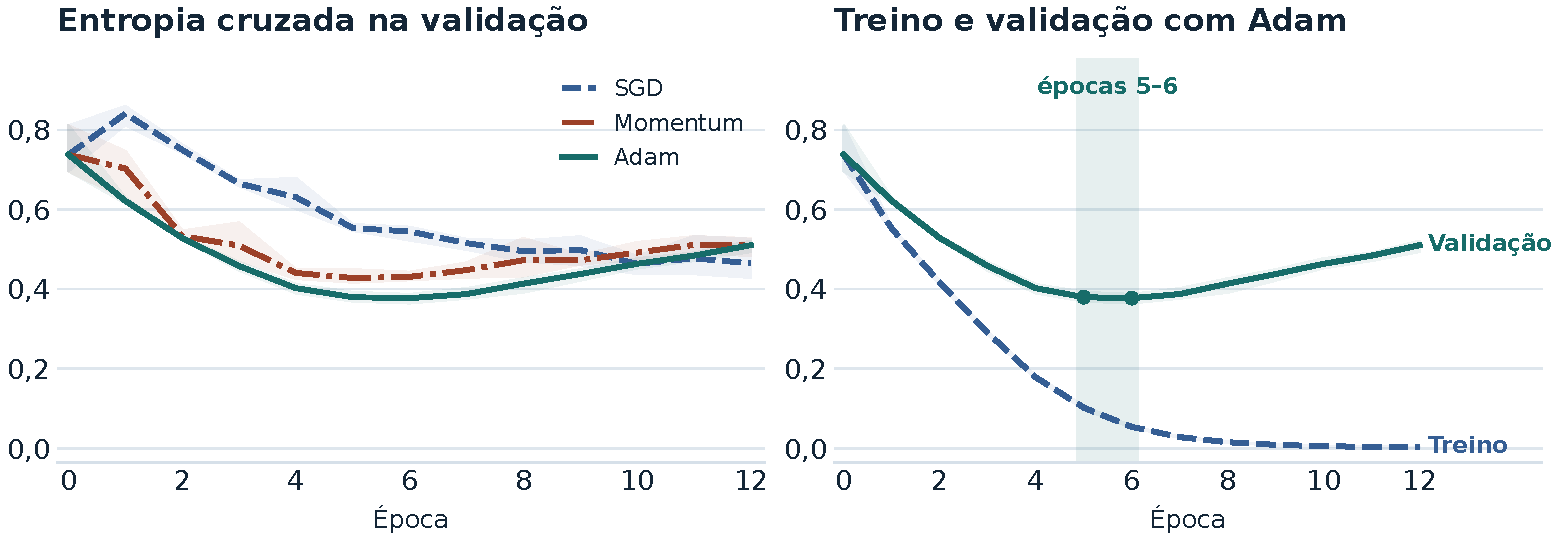
\includegraphics[width=\linewidth,height=.52\textheight,keepaspectratio]{figuras/otimizacao.pdf}
\par\raggedright\vspace{1mm}

Três taxas por método, 12 épocas e as mesmas partidas e minibatches por semente.
Escolhemos a menor CE de validação. Para Adam, os pesos guardados vieram das épocas 5 e 6.
\smallsource{Média e mínimo--máximo das sementes 17, 29 e 43.
\fonte{results/sequences/presentation_data.json}{Curvas salvas}.}
\end{frame}

% 06:40–07:50
\begin{frame}{Teste oficial do IMDb}
\begin{tabularx}{\linewidth}{@{}Xrrr@{}}
\toprule
Modelo & Acurácia & F1 macro & CE calibrada\\
\midrule
\LinhasTeste
\bottomrule
\end{tabularx}
\vspace{5mm}

O TF-IDF usa unigramas e bigramas do texto inteiro.
A CNN lê até 400 tokens e o BERT até 192 WordPieces.

Na CNN, a acurácia passa de 87,34\% até 100 palavras para 81,52\%
acima de 500.
\smallsource{25.000 resenhas. A temperatura foi ajustada em uma divisão separada.
\fonte{results/comparison.csv}{Métricas originais}.}
\end{frame}

% 07:50–09:00
\begin{frame}{Auditoria de palavras e BPE}
\begin{columns}[c,onlytextwidth]
\begin{column}{.51\textwidth}
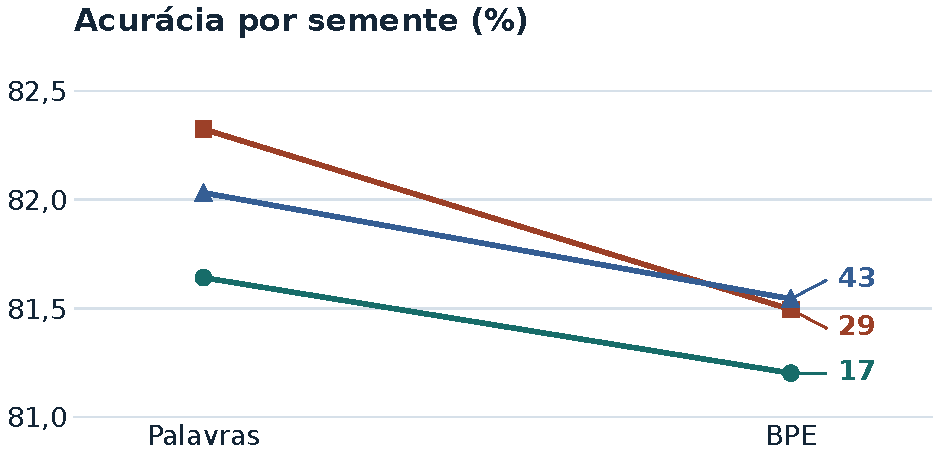
\includegraphics[width=\linewidth]{figuras/bpe_pareado.pdf}
\end{column}
\begin{column}{.45\textwidth}
{\large\strong{3,27\% \(\to\) 0\%}}\par
Tokens desconhecidos
\vspace{2mm}

{\large\strong{82,00\% \(\to\) 81,41\%}}\par
Acurácia média
\vspace{2mm}

As janelas contam tokens. Com subpalavras, podem cobrir menos palavras.
\end{column}
\end{columns}
\vspace{2mm}
Mesma CNN, três sementes pareadas e Adam a 0,001 nas duas receitas.
\smallsource{Auditoria BPE de 2.048 resenhas. Eixo vertical ampliado.
\fonte{results/bpe/audit_metrics.json}{Resultados por semente}.}
\end{frame}

% 09:00–10:10
\begin{frame}{Predições no par de contraste}
\begin{tabularx}{\linewidth}{@{}Xlrr@{}}
\toprule
Fim da resenha & Leitura planejada & CNN palavras & CNN BPE\\
\midrule
A. \textit{but it was wonderful} & Positiva & Neg. (\PalavrasA) & Neg. (\BPEA)\\
B. \textit{but it was terrible} & Negativa & Pos. (\PalavrasB) & Pos. (\BPEB)\\
\bottomrule
\end{tabularx}
\par\vspace{4mm}
\large
As seis CNNs mudaram de classe na direção oposta à leitura planejada.
\normalsize

No par com negação, houve troca de classe em duas sementes por palavras
e em uma semente com BPE.
\smallsource{Escore positivo médio entre parênteses, com três sementes por tokenizer.
\fonteatual{seminario/dados/pares_resultados.json}{Resultados dos quatro pares}.}
\end{frame}

% 10:10–11:30
\begin{frame}{Limite do máximo global}
\nota{\(S=\) \textit{I have a few thoughts about this movie.}}
\vspace{4mm}

\textbf{A}\quad \(S\) \enspace \textit{I loved the acting.}\enspace \(S\)
\enspace \textit{I hated the ending.}\enspace \(S\)

\textbf{B}\quad \(S\) \enspace \textit{I hated the ending.}\enspace \(S\)
\enspace \textit{I loved the acting.}\enspace \(S\)

\vspace{3mm}
O separador preserva as janelas de 3, 4 e 5 tokens quando os dois blocos trocam de lugar.
Cada filtro continua vendo as mesmas janelas e retorna o mesmo máximo.

\large\strong{Diferença máxima de logit igual a zero nos seis checkpoints.}
\smallsource{Controle sintético com igualdade verificada nas duas tokenizações.}
\end{frame}

% 11:30–12:00
\begin{frame}{Resultados e limites da CNN}
\Large
O que chega à camada final são os máximos de respostas locais.
\vspace{4mm}

\normalsize
Isso explica a sensibilidade à ordem dentro de uma janela
e a invariância quando as janelas se preservam.

No relatório, os pares mostram \emph{como} a rede erra.
A auditoria mede \emph{quanto} ela acerta no conjunto reservado.
\smallsource{\href{\projetourl}{Código, notebook, relatórios e evidências}.}
\end{frame}

% Bloco adicional, 12:00–13:30
\begin{frame}{Do IMDb aos comentários do YouTube}
\begin{tabularx}{.88\linewidth}{@{}>{\color{Teal}\bfseries}l@{\quad}>{\raggedright\arraybackslash\itshape}X@{}}
A & \ComentarioA\\
B & \ComentarioB\\
\end{tabularx}
\par\vspace{2mm}
\begin{tabular}{@{}lrr@{}}
\toprule
Comentário & CNN palavras & CNN BPE\\
\midrule
\LinhasYouTube
\bottomrule
\end{tabular}
\par\vspace{2mm}
As duas CNNs deram classe positiva. A comenta a repercussão do artista
e B pergunta pela reação do público. A opinião sobre a música fica em aberto.
\smallsource{Comentários de \textit{Baby}, sem rótulos de referência. Escore positivo da semente 17.
\fonteatual{seminario/dados/fora_dominio_resultados.json}{Resultados completos}.}
\end{frame}

% Bloco adicional, 13:30–15:00
\begin{frame}{Encoders e geração de texto}
\begin{tabularx}{\linewidth}{@{}Xrr@{}}
\toprule
Encoder & Cabeça treinada & Ajuste completo\\
\midrule
\LinhasRegimes
\bottomrule
\end{tabularx}
\par\vspace{3mm}

Os encoders geram vetores contextuais. Uma média mascarada alimenta a
cabeça linear. No ajuste completo, gradientes também chegam ao encoder.

\strong{Qwen3-8B.} No ensaio de geração, o modelo escreve uma avaliação
token a token. Comparamos o texto após alterar suas ativações.
\smallsource{Tabela com acurácia média, três sementes e 2.048 resenhas na auditoria sequencial.
\fonte{results/sequences/summary.json}{Encoders}.
\fonte{QWEN_EXPERIMENTO.md}{Geração com o Qwen}.}
\end{frame}

\appendix

\begin{frame}{Métricas por divisão}
\small
\begin{tabularx}{\linewidth}{@{}lXrrr@{}}
\toprule
Divisão & Modelo & Acurácia & F1 macro & CE bruta\\
\midrule
\LinhasOriginal
\bottomrule
\end{tabularx}
\smallsource{Apoio. Estudo original. \fonte{results/comparison.csv}{Resultados salvos}.}
\end{frame}

\begin{frame}{Comprimento e calibração}
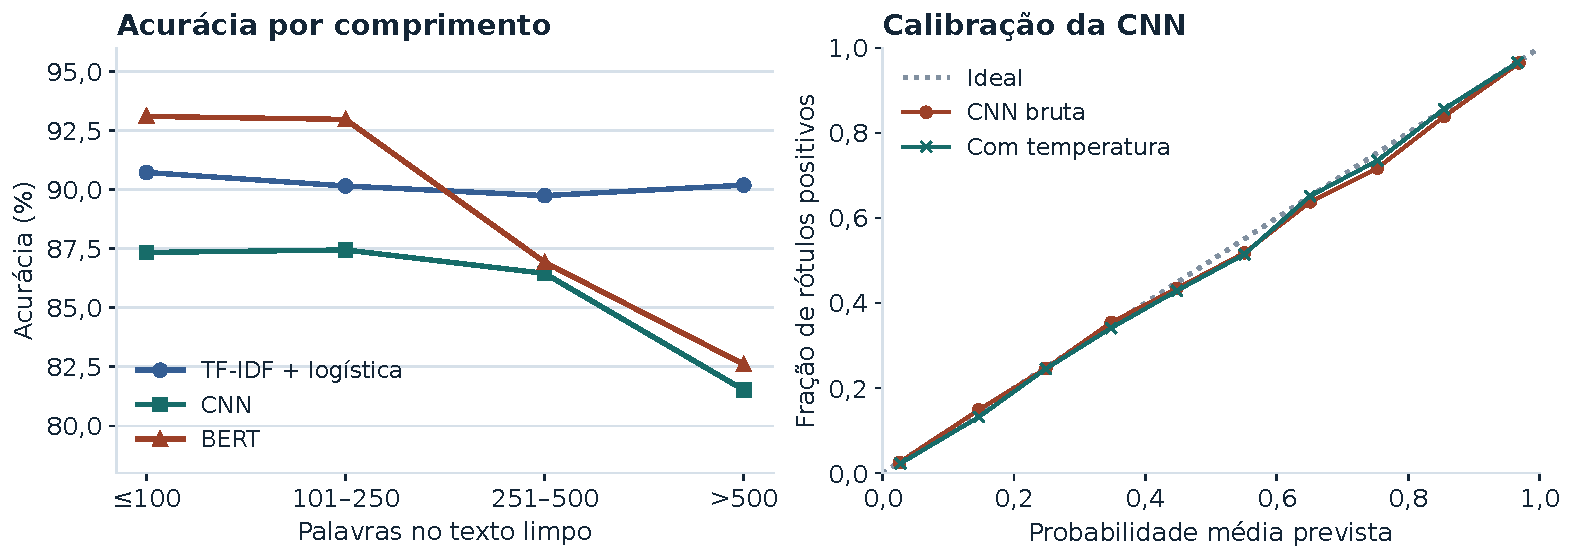
\includegraphics[width=\linewidth]{figuras/diagnostico_oficial.pdf}

Temperatura reescala a margem. Na CNN, a CE do teste foi de
0,3040 para 0,3037. A classificação usa o mesmo limiar.
\smallsource{Apoio. Teste oficial. \fonte{results/analysis/subgroup_metrics.csv}{Comprimento}
e \fonte{results/cnn/metrics.json}{calibração}.}
\end{frame}

\begin{frame}{Geração com o Qwen3-8B}
Em \textit{Signal 2040}, Bela encontra um teatro vazio e tenta organizar
uma apresentação com Evan. O prompt e o resumo \texttt{FACT} ficaram iguais.
\par\vspace{3mm}
\begin{tabularx}{\linewidth}{@{}rX@{}}
\toprule
\(\alpha\) & Opinião gerada em \texttt{REVIEW}\\
\midrule
\(-2\) & \textit{The film's direction lacks coherence and the pacing feels disjointed.}\\
\(0\) & \textit{The film's storytelling is engaging with a steady pace.}\\
\(+2\) & \textit{The film offers a thoughtful blend of gentle storytelling and warm performances.}\\
\bottomrule
\end{tabularx}
\par\vspace{3mm}
No bloco 28, somamos \(\alpha s v\) à ativação depois do marcador
\texttt{REVIEW}. Com \(\alpha=0\), a geração segue sem intervenção.
\smallsource{Apoio. Primeiro enredo sintético de teste.
\fonte{results/qwen_improved/presentation_examples.json}{Saídas integrais}.
\fonte{QWEN_EXPERIMENTO.md}{Direção e controles}.}
\end{frame}

\begin{frame}{Reprodução}
\begin{tabularx}{\linewidth}{@{}lX@{}}
\toprule
Material & O que permite conferir\\
\midrule
\fonte{notebooks/seminario_completo.ipynb}{Notebook único} & Arquitetura, tokenização, gradientes e estudos completos\\
\fonteatual{docs/RESULTADOS.md}{Tabelas} & Acurácia, F1 macro e CE por protocolo\\
\fonte{docs/PROTOCOLO_SEQUENCIAS.md}{CNN e encoders} & Grades, controles e escolha pela validação\\
\fonte{docs/PROTOCOLO_BPE.md}{BPE} & Tokenizer, seis pesos e auditoria pareada\\
\fonte{docs/CONEXOES_DISCIPLINA.md}{Mecanismos da disciplina} & MLPs, atalhos residuais e double descent\\
\bottomrule
\end{tabularx}
\par\vspace{4mm}
O JSON de pares preserva escores, IDs e janelas por semente.
\smallsource{Apoio. Os experimentos, condições descartadas e registros por semente
ficam no repositório.}
\end{frame}

\end{document}
